	\paragraph{QuizziPedia::Front-End::ModelViews::TrainingModelView}
	
	\label{QuizziPedia::Front-End::ModelViews::TrainingModelView}
	
	\begin{figure}[ht]
		\centering
		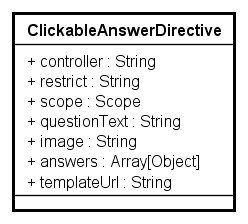
\includegraphics[scale=0.5,keepaspectratio]{UML/Classi/Front-End/QuizziPedia_Front-end_Templates_ClickableAnswerTemplate.png}
		\caption{QuizziPedia::Front-End::ModelViews::LoginModelView}
	\end{figure} \FloatBarrier
	
	\begin{itemize}
		\item \textbf{Descrizione}: classe di tipo modelview la cui istanziazione è contenuta all'interno della variabile di ambiente \$scope di \textit{Angular.js\ped{G}}. All'interno di essa sono presenti le variabili e i metodi necessari per il \textit{Two-Way Data-Binding\ped{G}} tra la view \texttt{TrainingView} e il controller \texttt{TrainingController};
		\item \textbf{Utilizzo}: viene utilizzata per effettuare il \textit{Two-Way Data-Binding\ped{G}} tra la view \texttt{TrainingView} e il controller \texttt{TrainingController} rendendo disponibili variabili e metodi;
		\item \textbf{Relazioni con altre classi}: 
		\begin{itemize}
			\item \textit{OUT} \texttt{TrainingView}: view principale della modalità allenamento, conterrà i vari templates di ogni domanda dell'allenamento; 
			\item \textit{OUT} \texttt{TrainingController}: questa classe permette di gestire la modalità allenamento sottoponendo all'utente le giuste domande adatte al suo livello;
		\end{itemize}
		\item \textbf{Attributi}: 
		\begin{itemize}
			\item \textit{+ topic: String} \\
			Attributo contenente l'argomento scelto dall'utente per l'allenamento;
			\item \textit{+ keywords: Array[String]}\\
			Attributo contenente l'\texttt{array} di keywords scelte dall'utente per l'allenamento;
		\end{itemize}
		\item \textbf{Metodi}: 
		\begin{itemize}
			\item \texttt{+} \texttt{addQuestion(question: QuestionItemModel): void} \\
			Metodo che gestisce l'evento per inserire una domanda nella cronologia delle domande. \\
			\textbf{Parametri}:
			\begin{itemize}
				\item \texttt{question: QuestionItemModel} \\
				Parametro contenente un riferimento all'oggetto di tipo \texttt{QuestionItemModel};
			\end{itemize}
			\item \texttt{+} \texttt{loadNewQuestionBy(topic: String, keywords: Array[String], level: Number): void} \\
			Metodo che emette l'evento per scaricare una nuova domanda in base ai parametri passati. \\
			\textbf{Parametri}:
			\begin{itemize}
				\item \texttt{topic: String} \\
				Parametro contenente l'argomento della domanda;
				\item \texttt{keywords: Array[String]} \\
				Parametro contenente un\texttt{array} di stringhe che rappresenta le keywords scelte per l'allenamento;
				\item \texttt{level: Number} \\
				Parametro contenente il livello dell'utente;
			\end{itemize}
		\end{itemize}
	\end{itemize}
	
	